\chapter{Game Theory}
\label{chap:game-theory}

\begin{lemma}
	For every game $G$, there exists at least one individually rational strategy profile.
	In other words, $\mathcal{S}_1(G) \ne \emptyset$.
\end{lemma}

\begin{proof}
	For every player $i \in P$ we denote $m_i \in S_i$ the strategy that lower-bounds utility of player $i$:
	\[
		m_i = \text{arg} \max_{t_i \in S_i} \min_{\vect_{-i} \in S_{-i}} u_i(t_i, \vect_{-i}).
	\]
	We claim that the strategy profile $\mm = (m_1, \dots, m_n) \in S$ is individually rational.
	If $\mm$ was not individually rational, there would have to be some player $j \in P$ and a strategy $s_j^* \in S_j$ that would ensure a better worst-case payoff: $\min_{\vecs_{-j} \in S_{-j}}u_j(s_j^*, \vecs_{-j}) > u_j(\mm)$ which would contradict the choice of~$m_j$.
\end{proof}

In this chapter, we introduce two new equilibria: the perfectly transparent best response equilibrium, and the perfectly transparent optimal profile equilibrium.
Then, we discuss some relations between these two equilibiria, and between the other equilibria introduced in \autoref{chap:background}.

\begin{definition}[Perfectly transparent best response]
	In a game (possibly with ties) $G = (P, S, \uu)$ we say a strategy $s_i^* \in S_i$ is a perfectly transparent best response to a strategy profile $\vecs_{-i} \in S_{-i}$ of the opponent players if it is the Nashian best response to $\vecs_{-i}$ across all profiles that survive the maximum possible number of preemption rounds.
	The weak/strict notion is inherited from the Nashian best response.
	Formally $s_i^*$ is a (\textit{weak}) perfectly transparent best response if either $(s_i^*, \vecs_{-i})$ is a PTE or $\exists k \in \N: (s_i^*, \vecs_{-i}) \in \mathcal{S}_k(G), (s_i, \vecs_{-i}) \notin \mathcal{S}_{k+1}(G) \forall s_i \in S_i$, and
	\[
		\forall (s_i', \vecs_{-i}) \in \mathcal{S}_k(G): u_i(s_i^*, \vecs_{-i}) \ge u_i(s_i', \vecs_{-i}).
	\]
	It is a \textit{strict} perfectly transparent best response if either $(s_i^*, \vecs_{-i})$ is a PTE or $\exists k \in \N: (s_i^*, \vecs_{-i}) \in \mathcal{S}_k(G), (s_i, \vecs_{-i}) \notin \mathcal{S}_{k+1}(G) \forall s_i \in S_i$, and
	\[
		\forall (s_i', \vecs_{-i}) \in \mathcal{S}_k(G): s_i' \ne s_i^* \implies u_i(s_i^*, \vecs_{-i}) > u_i(s_i', \vecs_{-i}).
	\]
\end{definition}

\begin{definition}[Perfectly transparent best response equilibrium]
	We say a strategy profile $\vecs = (s_1, \dots, s_n) \in S$ is a (\textit{weak}) perfectly transparent best response equilibrium (PTBRE) if $s_i$ is a (weak) perfectly transparent best response to $\vecs_{-i}$ for all players $i \in P$.
	
	Similarly, $\vecs$ is a \textit{strict} PTBRE if $s_i$ is a strict perfectly transparent best response to $\vecs_{-i}$ for all players $i \in P$.
\end{definition}

\begin{definition}[Perfectly transparent $i$-best profile]
	For a game $G = (P, S, \uu)$ of two players with $P = \{i, j\}$
	we say a strategy profile $\vecs = (s_1, s_2) \in S$ is a (\textit{weak}) perfectly transparent $i$-best profile if
	$j$'s strategy $s_j$ is a (weak) perfectly transparent best response to $s_i$, and
	\[
		\forall s_i' \in S_i: u_i(\vecs) \ge u_i\left(s_i', b(s_i')\right),
	\]
	where $b(s_i')$ is some weak perfectly transparent best response of player $j$ to $s_i'$ (note that there may be multiple best responses to $s_i'$ but they must all have the same utility for player $i$).

	It is a \textit{strict} perfectly transparent $i$-best profile if $s_j$ is a strict perfectly transparent best response to $s_i$ and
	\[
		\forall s_i' \in S_i: s_i' \ne s_i \implies u_i(\vecs) > u_i\left(s_i', b(s_i')\right).
	\]
	Note that even in the strict definition, we still consider $b(s_i')$ to be a weak best response.
	This is to ensure that every strict best profile is also a weak best profile.
\end{definition}

\begin{definition}[Perfectly transparent best profile equilibrium]
	For a game of two players, we say that a strategy profile $\vecs \in S$ is a (\textit{weak}) perfectly transparent best profile equilibrium (PTBPE) if $\vecs$ is a (weak) perfectly transparent $i$-best profile for both players $i \in P$.

	Similarly, $\vecs$ is a \textit{strict} PTBPE if it is a strict perfectly transparent $i$-best profile for both $i \in P$.
\end{definition}

\begin{definition}[Perfectly transparent $i$-optimal profile]
	For a given game $G = (P, S, \uu)$ and player $i \in P$ we say a strategy profile $\vecs = (s_1, \dots, s_n) \in S$ is a (\textit{weak}) perfectly transparent $i$-optimal profile if
	$s_i$ is a (weak) perfectly transparent best response to $\vecs_{-i}$ and
	\[
		\forall \vecs'_{-i} \in S_{-i}: u_i(\vecs) \ge u_i\left(b(\vecs'_{-i}), \vecs'_{-i}\right),
	\]
	where $b(\vecs'_{-i})$ is some weak perfectly transparent best response to $\vecs'_{-i}$ (note that there may be multiple best responses to $\vecs'_{-i}$ but they must all have the same utility for player $i$).

	It is a \textit{strict} perfectly transparent $i$-optimal profile if $s_i$ is a strict perfectly transparent best response to $\vecs_{-i}$ and
	\[
		\forall \vecs_{-i}' \in S_{-i}: \vecs_{-i}' \ne s_{-i} \implies u_i(\vecs) > u_i\left(b(\vecs_{-i}'), \vecs_{-i}'\right).
	\]
	Note that even in the strict definition, we still consider $b(\vecs_{-1})$ to be a weak best response.
	This is to ensure that every strict optimal profile is also a weak optimal profile.
\end{definition}

\begin{definition}[Perfectly transparent optimal profile equilibrium]
	We say that a strategy profile $\vecs \in S$ is a (\textit{weak}) perfectly transparent optimal profile equilibrium (PTOPE) if $\vecs$ is a (weak) perfectly transparent $i$-optimal profile for all $i \in P$.

	Similarly, $\vecs$ is a \textit{strict} PTOPE if it is a strict perfectly transparent $i$-optimal profile for all $i \in P$.
\end{definition}

Recall that for any game $G = (P, S, \uu)$, a strategy profile $\vecs \in S$ is individually rational if and only if it survives the first preemption round: $\vecs \in \mathcal{S}_1(G)$.
This means that every PTE must be individually rational.
If we think of these equilibiria as sets of strategy profiles in any possible game, we can express this as PTE $\subset$ IR.
It is not hard to see that the inclusion is indeed strict as there are games in which $\mathcal{S}_2 \subsetneq \mathcal{S}_1$, so not all individually rational profiles are PTEs.

In the rest of this chapter, we present several such inclusion results that help to understand the relations between individal rationality, perfetcly transparent best response equilibiria, perfectly transparent equilibiria, perfectly transparent optimal profile equilibiria, and minimax rationalizibility.


\section{Games with ties}

We start by presenting results about the most general setup: games with ties.
All the proofs presented in this section naturally hold also for the more specific cases (symmetric games, games without ties).
The results are summarized by a Venn diagram in \autoref{fig:venn-with-ties}.

\begin{figure}[b]
	\centering
	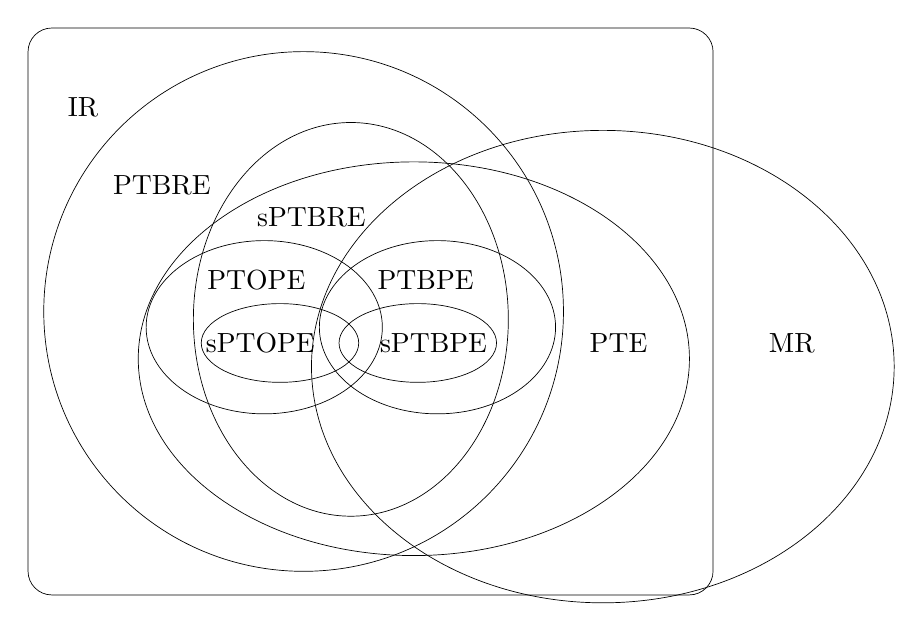
\begin{tikzpicture}[line width=0.25pt]
		\draw (0,0) ellipse (1 and 0.5);
		\draw (-0.2,0.2) ellipse (1.5 and 1.1);
		\draw (1.75,0) ellipse (1 and 0.5);
		\draw (2,0.2) ellipse (1.5 and 1.1);
		\draw (0.9,0.3) ellipse (2 and 2.5);
		\draw (0.3,0.4) ellipse (3.3 and 3.3);
		\draw (1.7,-0.2) ellipse (3.5 and 2.5);
		\draw[rounded corners=2ex] (-3.2,4) rectangle (5.5,-3.2);
		\draw (4.1,-0.3) ellipse (3.7 and 3);
		\node at (-0.25,0) {sPTOPE};
		\node at (-0.3,0.8) {PTOPE};
		\node at (1.95,0) {sPTBPE};
		\node at (1.85,0.8) {PTBPE};
		\node at (0.4,1.6) {sPTBRE};
		\node at (-1.5,2.0) {PTBRE};
		\node at (4.3,0) {PTE};
		\node at (-2.5,3) {IR};
		\node at (6.5,0) {MR};
	\end{tikzpicture}
	\caption{A Venn diagram depicting the inclusion of different equilibria in games with ties.}
	\label{fig:venn-with-ties}
\end{figure}

\begin{observation}
	\label{th:strict-sub-weak}
	We can see from our definition of PTOPE, PTBPE, and PTBRE that any strategy profile satisfying the strict definition of each equilibrium also satisfies the weak definition of the respective equilibrium.
	Thus, we have sPTOPE $\subset$ PTOPE, sPTBPE $\subset$ PTBPE, and sPTBRE $\subset$ PTBRE.
\end{observation}

\begin{remark}
	The inclusions are indeed strict, as shown in \autoref{tab:ptope-not-sub-sptope}, TODO, and TODO.
\end{remark}

\begin{observation}
	\label{th:ptope-subset-ptbre}
	For any game $G = (P, S, \uu)$, if a strategy profile $\vecs \in S$ is a PTOPE, then it is a PTBRE.
	Similarly, if $\vecs$ is a strict PTOPE, then it is a strict PTBRE.
	Thus, we have PTOPE $\subset$ PTBRE, and sPTOPE $\subset$ sPTBRE.
\end{observation}

\begin{proof}
	If $\vecs$ is a PTOPE, it is by definition a perfectly transparent $i$-optimal profile for every player $i \in P$.
	If $\vecs$ is a perfectly transparent $i$-optimal profile, then, again by definition, $s_i$ is a perfectly transparent best response to $\vecs_{-i}$.
	This being true for all $i \in P$ is exactly the definition of a PTBRE.
	The same argument holds for strict equilibiria.
\end{proof}

\begin{remark}
	TODO: inclusion indeed strict
\end{remark}

\begin{remark}
	\autoref{tab:PTOPE-not-sub-sptbre} shows that PTOPE $\not\subseteq$ sPTBRE.
\end{remark}

\begin{lemma}
	\label{th:ptope-subset-pte}
	If a game $G = (P, S, \uu)$ has a PTOPE $\vecs \in S$, then $\vecs$ is also a PTE, i.e., we have the inclusion PTOPE $\subset$ PTE.
\end{lemma}

\begin{proof}
	For the sake of deriving a contradiction, suppose that there is a game $G = (P, S, \uu)$ with a strategy profile $\vecs = (s_1, \dots, s_n) \in S$ such that $\vecs$ is a PTOPE but not a PTE and let $k$ be the last preemption round in which $\vecs$ is not eliminated (i.e., $\vecs \in \mathcal{S}_k(G)$ but $\vecs \notin \mathcal{S}_{k+1}(G)$).
	Because $\vecs$ is eliminated in the $(k+1)$\textsuperscript{st} round, there must be some player $i \in P$ with a strategy $s_i^* \ne s_i$ which causes the elimination:
	\[
		\forall \vecs_{-i}' \in S_{-i}: (s_i^*, \vecs_{-i}') \in \mathcal{S}_k(G) \implies u_i(s_i^*, \vecs_{-i}') > u_i(\vecs).
	\]
	Let $\vecs_{-i}^* \in S_{-i}$ be the opponents' profile that minimizes $u_i(s_i^*, \vecs_{-i}^*)$, subject to $(s_i^*, \vecs_{-i}^*)\in \mathcal{S}_k(G)$ (there must be at least one such profile to cause $\vecs \notin \mathcal{S}_{k+1}(G)$).
	Let $b \in S_i$ be the perfectly transparent best response to $\vecs_{-i}^*$.
	By the choice of $\vecs_{-i}^*$, we must have $u_i(b, \vecs_{-i}^*) \ge u_i(s_i^*, \vecs_{-i}^*) > u_i(\vecs)$.
	This means that $\vecs$ is not a perfectly transparent $i$-optimal profile, contradicting $\vecs$ being a PTOPE.
\end{proof}

\begin{remark}
	\autoref{tab:pte-ne-PTOPE} shows that the inclusion is strict.
\end{remark}

\begin{lemma}
	\label{th:ptbpe-subset-pte}
	If a game $G = (P, S, \uu)$ of two players has a PTBPE $\vecs \in S$, then $\vecs$ is a PTE; we have PTBPE $\subset$ PTE.
\end{lemma}

\begin{proof}
	The proof is very similar to the proof of \autoref{th:ptope-subset-pte}.
	We suppose for the sake of contradiction that there is a game $G = (P, S, \uu)$ with $P = \{1, 2\}$, and a strategy profile $\vecs = (s_1, s_2) \in S$ such that $\vecs$ is a PTBPE but not a PTE and let $k$ be the last preemption round in which $\vecs$ is not eliminated (i.e., $\vecs \in \mathcal{S}_k(G)$ but $\vecs \notin \mathcal{S}_{k+1}(G)$).
	Because $\vecs$ is eliminated in the $(k+1)$\textsuperscript{st} round, there must be some player $i \in P$ with a strategy $s_i^* \ne s_i$ which causes the elimination:
	\[
		\forall s_j' \in S_j: (s_i^*, s_j') \in \mathcal{S}_k(G) \implies u_i(s_i^*, s_j') > u_i(\vecs),
	\]
	where $j = 3 - i$ is the opponent of $i$ and there is at least one $s_j' \in S_j$ which satisfies $(s_i^*, s_j') \in \mathcal{S}_k(G)$.
	Let $b \in S_j$ be the perfectly transparent best response of player $j$ to $s_i^*$.
	We must have $(s_i^*, b) \in \mathcal{S}_k$ and so $u_i(s_i^*, b) > u_i(\vecs)$.
	This means that $\vecs$ is not a perfectly transparent $i$-best profile, contradicting $\vecs$ being a PTBPE.
\end{proof}

\begin{lemma}
	\label{th:ptbpe-subset-ptbre}
	If a game $G = (P, S, \uu)$ of two players has a PTBPE $\vecs \in S$, then $\vecs$ is a PTBRE.
	Similarly, if $\vecs$ is a strict PTBPE, then it is a strict PTBRE.
	We have PTBPE $\subset$ PTBRE, and sPTBPE $\subset$ sPTBRE.
\end{lemma}

\begin{proof}
	Suppose that a game $G = (P, S, \uu)$ with $P = \{i, j\}$ has a PTBPE $\vecs = (s_i, s_j) \in S$.
	By definition, this means that $\vecs$ is a perfectly transparent $i$-best profile, hence $s_j$ is a perfectly transparent best response to $s_i$.
	Moreover, $\vecs$ is a perfectly transparent $j$-best profile, hence $s_i$ is a perfectly transparent best response to $s_j$.
	This implies that $\vecs$ is a PTBRE.
	The same argument holds for strict equilibiria.
\end{proof}

\begin{observation}
	\label{th:pte-subset-ir}
	In any game $G = (P, S, \uu)$, if a strategy profile $\vecs \in S$ is a PTE, then it is individually rational.
	We have PTE $\subset$ IR.
\end{observation}

\begin{proof}
	By definition, a profile is IR if it survives the first preemption round, i.e., $\vecs \in \mathcal{S}_1$.
	If $\vecs$ is a PTE, it survives all preemption rounds.
	Thus, it must satisfy $\vecs \in \mathcal{S}_1$.
\end{proof}

\begin{lemma}
	\label{th:ptbre-subset-ir}
	For any game $G = (P, S, \uu)$, if a strategy profile $\vecs \in S$ is a PTBRE, then it is individually rational.
	Thus, we have PTBRE $\subset$ IR.
\end{lemma}

\begin{proof}
	Let us suppose that there is a game $G = (P, S, \uu)$ and a strategy profile $\vecs = (s_1, \dots, s_n) \in S$ such that $\vecs$ is a PTBRE but not individually rational.
	This is equivalent to $s_i$ being a perfectly transparent best response to $\vecs_{-i}$ for all $i \in P$, and $\vecs \notin \mathcal{S}_1(G)$.
	Note that we must also have $(s_i', \vecs_{-i}) \notin \mathcal{S}_1(G)\ \forall s_i' \in S_i,\ \forall i \in P$ because otherwise $s_i$ would not be a perfectly transparent best response to $\vecs_{-i}$ for some player $i$.
	This means the perfetcly transparent best response of every player $i \in P$ to $\vecs_{-i}$ is simply a Nashian best response (since all considered strategy profiles are eliminated in the same preemption round).
	Thus, $\vecs$ is a Nash equilibrium, which is always individually rational.
\end{proof}

\begin{remark}
	\autoref{tab:ir-ne-ptbre} shows that the inclusion is indeed strict.
\end{remark}

Minimax rationalizibility intersects with all the other equilibiria, as shown in \autoref{tab:PTOPE-ne-minimax} and \autoref{tab:PTOPE-eq-minimax}.

\begin{lemma}
	\label{th:ptbpe-subset-mr}
	In any game $G = (P, S, \uu)$ of two players with $P = \{i, j\}$, if a strategy profile $\vecs \in S$ is a PTBPE, then it is minimax rationalizable.
	We have PTBPE $\subset$ MR.
\end{lemma}

\begin{proof}
	Suppose for the sake of contradiction that there is a strategy profile $\vecs \in S$ which is a PTBPE but not MR.
	This means there is some $k \in \N$ such that $\vecs \in \mathcal{R}_k$ and $\vecs \notin \mathcal{R}_{k+1}$.
	Suppose WLOG that player $i$ caused the elimination of $\vecs$ in the $k+1$\textsuperscript{st} round.
	This means, player $i$ has some strategy $s_i' \in S_i'$ such that
	\[
		\forall (s_i', s_j') \in \mathcal{R}_k: u_i(s_i', s_j') > u_i(\vecs),
	\]
	and there is at least one $s_j' \in S_j$ such that $(s_i', s_j') \in \mathcal{R}_k$.
	Now, we can observe that $(s_i', s_j) \in \mathcal{R}_k$; otherwise either the whole row or column corresponding to $(s_i', s_j)$ would have to be eliminated in some previous round but we know that $\vecs \in \mathcal{R}_k$ and $(s_i', s_j') \in \mathcal{R}_k$ for some $s_j' \in S_j$.
	Since $u_i(s_i', s_j) > u_i(\vecs)$, it cannot be that $s_i$ is a perfectly transparent best response to $s_j$. Hence, $\vecs$ cannot be a perfectly transparent $j$-best profile, a contradiction.
\end{proof}


\section{Games without ties}
We can observe that in games without ties, similar to Nash equilibria, weak and strict equilibiria are equivalent also in the case of PTBRE and PTOPE.
Thus, in this section, we do not distingiush between them.
Moreover, all the \enquote{is subset of} relations are inherited from the previous section.
The only difference is that PTE is not intersecting with PTBRE anymore (the example in \autoref{tab:ties-pte-not-sub-ptbre} indeed has ties).

\begin{observation}
	\label{th:pte-subset-ptbre}
	If a strategy profile is a PTE, then it must be a PTBRE because in the last preemption round, there is only one strategy profile to choose from.
	We have PTE $\subset$ PTBRE.
\end{observation}

\begin{remark}
	\autoref{tab:ptbre-ne-pte} shows that the inclusion is strict.
\end{remark}

All inclusions for games without ties are depicted by a Venn diagram in \autoref{fig:venn-general-without-ties}.

\begin{figure}[h]
	\centering
	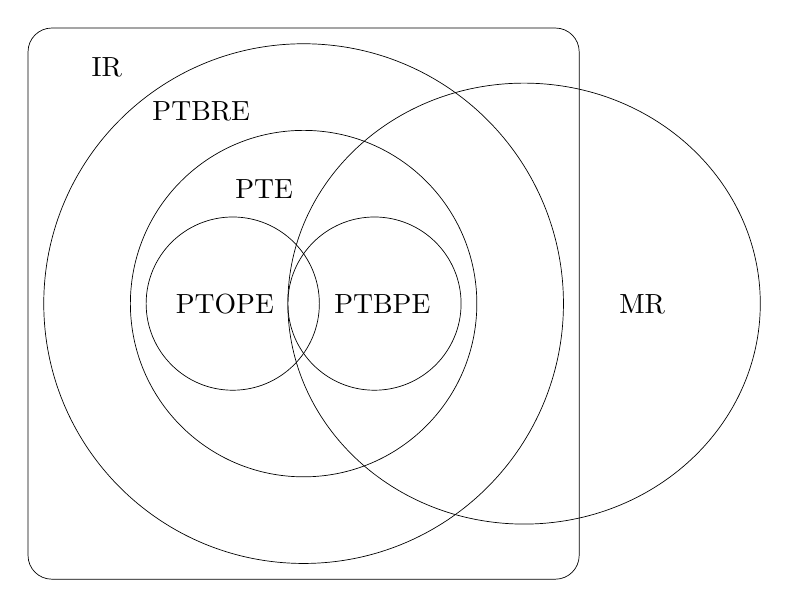
\begin{tikzpicture}[line width=0.25pt]
		\draw (-0.9,0) ellipse (1.1 and 1.1);
		\draw (0.9,0) ellipse (1.1 and 1.1);
		\draw (0,0) circle (2.2);
		\draw (0,0) circle (3.3);
		\draw[rounded corners=2ex] (-3.5,3.5) rectangle (3.5,-3.5);
		\draw (2.8,0) ellipse (3 and 2.8);
		\node at (-1,0) {PTOPE};
		\node at (1,0) {PTBPE};
		\node at (-0.5,1.45) {PTE};
		\node at (-1.3,2.45) {PTBRE};
		\node at (-2.5,3.0) {IR};
		\node at (4.3,0) {MR};
	\end{tikzpicture}
	\caption{A Venn diagram depicting the inclusion of different equilibria in games without ties.}
	\label{fig:venn-general-without-ties}
\end{figure}


\section{Symmetric games without ties}
In this section, we restrict ourselves to symmetric games without ties.
All the \enquote{subset} relations from the previous section still hold, since symmetric games are a special case of general games.
Moreover, none of the equilibiria collapses (i.e., they are still strict subsets, even when restricted to symmetric games); this because all the provided counterexamples are symmetric games.
The only new relation that emerges is between minimax rationaliziblity and~PTE.
All the inclusions are depicted in \autoref{fig:venn-sym-without-ties}.
Furthermore, we present some other interesting observations about symmetric games.

\begin{figure}
	\centering
	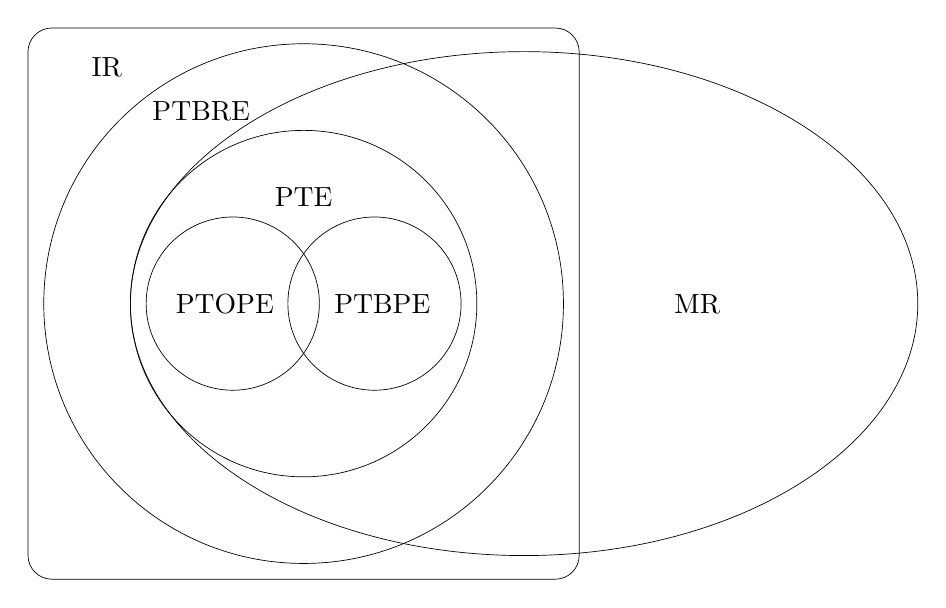
\begin{tikzpicture}[line width=0.25pt]
		\draw (-0.9,0) ellipse (1.1 and 1.1);
		\draw (0.9,0) ellipse (1.1 and 1.1);
		\draw (0,0) circle (2.2);
		\draw (0,0) circle (3.3);
		\draw[rounded corners=2ex] (-3.5,3.5) rectangle (3.5,-3.5);
		\draw (2.8,0) ellipse (5 and 3.2);
		\node at (-1,0) {PTOPE};
		\node at (1,0) {PTBPE};
		\node at (-0,1.35) {PTE};
		\node at (-1.3,2.45) {PTBRE};
		\node at (-2.5,3.0) {IR};
		\node at (5,0) {MR};
	\end{tikzpicture}
	\caption{A Venn diagram depicting the inclusion of equilibria in symmetric games without ties.}
	\label{fig:venn-sym-without-ties}
\end{figure}

\begin{observation}
	 In a symmetric game $G = (P, S, \uu)$, if a strategy profile $\vecs \in S$ is a PTE, then it lies on the diagonal, i.e., we have $\vecs = (a, a, \dots, a)$ for some strategy $a$.
\end{observation}

\begin{proof}
	If there was a PTE somewhere else than on the diagonal, we would necessarily have multiple PTEs by symmetry, contradicting the uniqueness of PTE.
\end{proof}

\begin{corollary}
	If a symmetric game $G = (P, S, \uu)$ has a PTE $\vecs \in S$ and $\vecs$ is the perfectly transparent $i$-optimal profile for some player $i \in P$, then $\vecs$ is a PTOPE. 
\end{corollary}

\begin{proof}
	Since $\vecs$ is on the diagonal and it is the perfectly transparent $i$-optimal profile for some $i \in P$, by symmetry, it must actually be the perfectly transparent $j$-optimal profile for all $j \in P$, which is the definition of PTOPE.
\end{proof}

\begin{lemma}[Fourny \cite{Fourny20}]
	\label{th:pte-sym-subset-mr}
	In a symmetric game $G = (P, S, \uu)$, if a strategy profile $\vecs \in S$ is a PTE, then it is minimax rationalizable.
	Thus, we have PTE\textsuperscript{sym} $\subset$ MR\textsuperscript{sym}.
\end{lemma}

\begin{proof}
	Suppose for the sake of deriving a contradiction that there is a game $G = (P, S, \uu)$ and a strategy profile $\vecs \in S$ that is a PTE but not minimax rationalizable.
	By definition, this means that there is some player $i \in P$ such that $(s_i, \vecs_{-i}')$ is not minimax rationalizable for any $\vecs' \in S$.
	By symmetry, if this statement holds for one player, then it must hold for all players.
	Let $s_j$ be the strategy that minimax-dominates $s_i$ (i.e. causes that $s_i$ is not minimax rationalizable).
	We denote $\vecs^* = (s_j, s_j, \dots, s_j)$.
	In the round where strategy $s_i$ is eliminated, strategy profile $\vecs^*$ must survive---otherwise strategy $s_j$ would be eliminated as well, but we supposed that $s_j$ is the strategy that caused the elimination of $s_i$.
	Moreover, we must have $u_i(\vecs^*) > u_i(\vecs)\ \forall i \in P$ because $s_j$ minimax-dominates $s_i$.
	This means $\vecs$ is not Pareto-optimal which contradicts $\vecs$ being a PTE.
\end{proof}

\begin{remark}
	\autoref{tab:sym-mr-ne-pte} shows that the inclusion is strict.
\end{remark}

\begin{remark}
	\autoref{tab:sym-ptbre-ne-mr} and \autoref{tab:sym-mr-ne-ptbre} show that PTBRE and MR are still intersecting, even in symmetric games.
\end{remark}
